\documentclass{beamer}

\usepackage{ctex}
\usepackage{graphicx}
\usepackage{animate}

\usetheme{Pittsburgh}

\graphicspath{{pictures/}}

% \usecolortheme{dove} % 

% 最传统 warsaw Pittsburgh Singapore Malmoe Boadilla


\title[Latex使用模板]{蒙古高原生态退化与机理分析研究}
\subtitle[课程]{硕士论文中期汇报}
\author[Dong Yu]{{\small 学生 董昱 \\ 导师{ }闫慧敏{ }副研究员}}
\date[\today]{\today}
\institute[中科院地理所]{中国科学地理科学与资源研究所\par 中国科学院大学}
% \titlegraphic{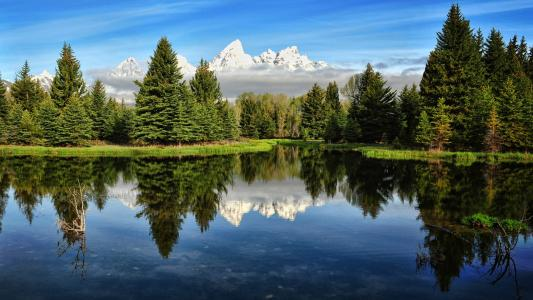
\includegraphics[width=0.17\textwidth]{image.jpg}}

\begin{document}
	
	% 标题页帧
	\frame{\titlepage}

	\begin{frame}[label = outline]
		\frametitle{汇报内容}
		% \tableofcontents[part=1,pausesections]
		\tableofcontents
	\end{frame}

	\section{研究意义与文献综述}

	\begin{frame}[c] % c表示对齐方式
		\frametitle{研究意义}
        在蒙古高原地区:
        \par
        \par
		\begin{enumerate}
			\item 什么是草地退化?
			\item 什么地区发生了草地退化?(退化识别)
			\item 为什么发生草地退化?(退化机理)
		\end{enumerate}
		
		% \hyperlink{outline}{\beamergotobutton{超链接}}
	\end{frame}

    
	\begin{frame}[c] % c表示对齐方式
		\frametitle{研究意义}
		% \framesubtitle{也许会用到这个副标题}
		
	\end{frame}

	\section{学位论文研究进展}
	
	\subsection{下一步论文工作计划}
	
	\begin{frame}[c] % c表示对齐方式
		\frametitle{动画}

		\animategraphics[autoplay,loop,controls,width=.7\textwidth,height=.7\textheight]{1}{test}{0}{2}  

	\end{frame}


	\section{预期成果及其创新性}
	
	\begin{frame}
		\begin{columns}
			\column{.5\textwidth}
			First column text and/or code
			\column{.5\textwidth}
			Second column text and/or code
		\end{columns}
	\end{frame}

\end{document}